\subsection{External ADC reference voltage} \label{subsec:5VREF}

The \SIQ{5}{\volt} external reference for the ADC is being generated by the precision REF02 voltage reference shown on the schematic on figure \refq{fig_7_1_3_REF}. 

\begin{figure}[H]
    \centering
    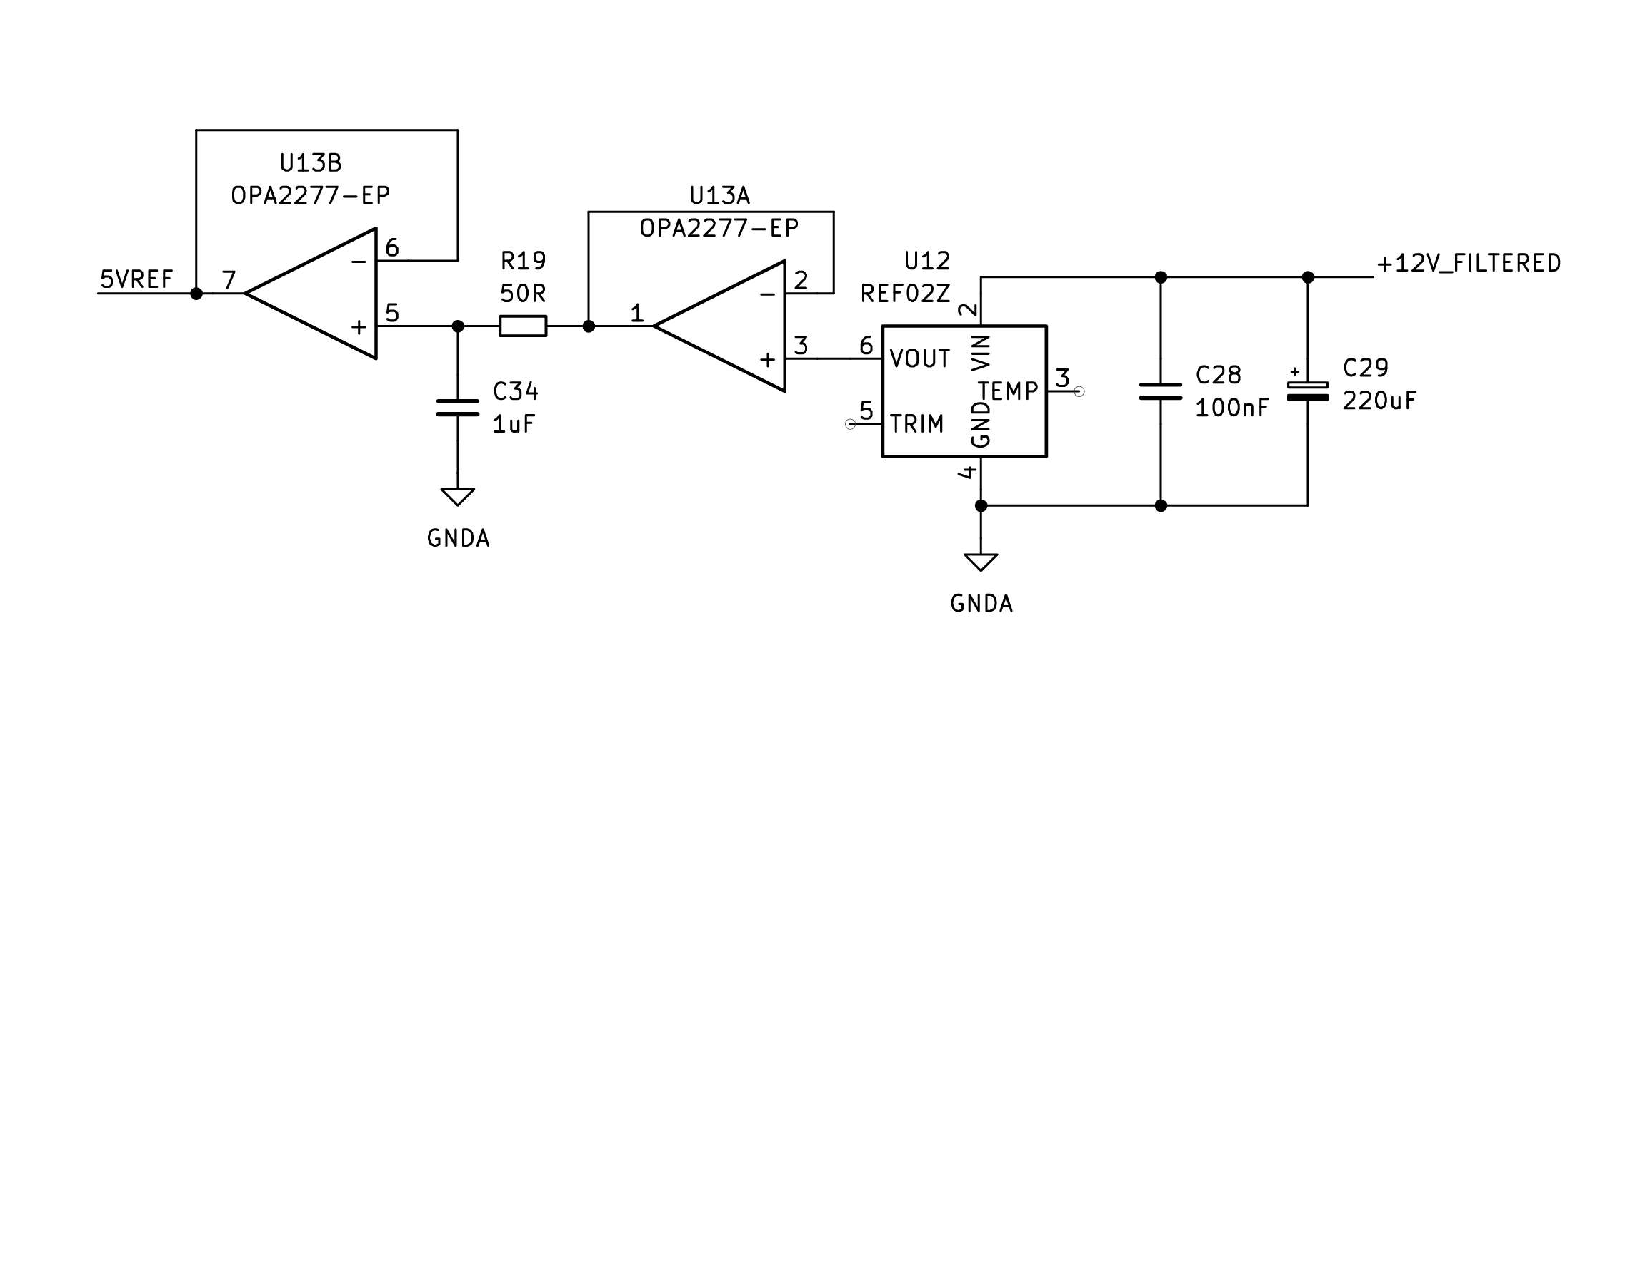
\includegraphics[clip, trim=0 300 0 0, width=1\textwidth]{Sections/7_SystemDesign/Figures/7_1_3_REF.pdf}
    \caption{The 5V reference is being generated by a REF02 voltage reference\cite{REF02}. A simple 1-pole is added to attenuate wideband noise.}
    \label{fig_7_1_3_REF}
\end{figure}

The REF02 voltage reference has $\pm 0.3\%$ output voltage accuracy along with $8.5 ppm / \degree C$ temperature stability. The output voltage of the reference will be in the interval $4.985 < V_O < 5.015$. The MCU may take this into account when analyzing the samples, however as both the current sampling and voltage sampling ADC will see the same offset, it is insignificant in this application. The REF02 has a trim input that could be used for calibrating the reference, but this will not be used for this project and the input is left floating.

According to the datasheet REF02 will produce wideband noise, this has not been verified during this project, as can be seen the graph on figure  \refq{fig_7_1_3_REFNOISE}.
\begin{figure}[H]
    \centering
    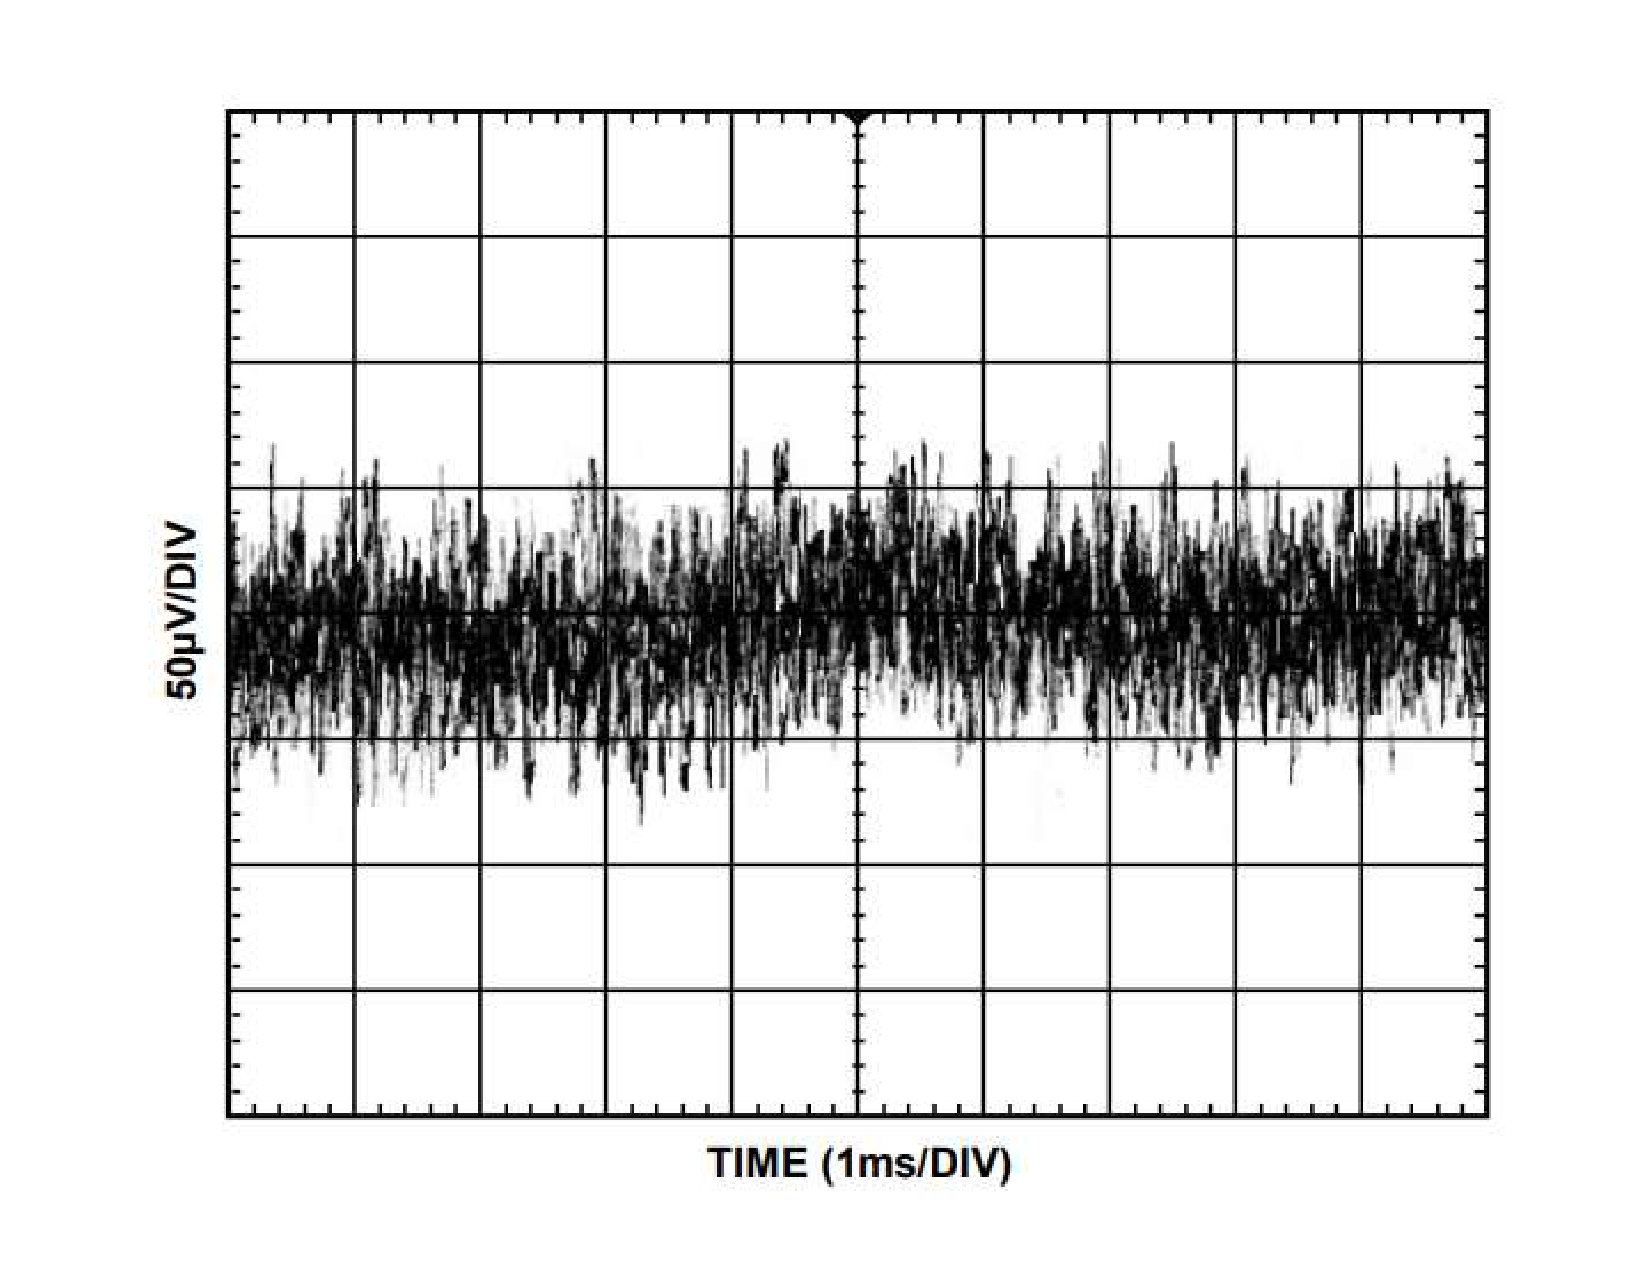
\includegraphics[clip, trim=0 25 0 0, width=0.6\textwidth]{Sections/7_SystemDesign/Figures/7_1_3_REFNoise.pdf}
    \caption{The REF02 voltage reference will generate noise at the output.}
    \label{fig_7_1_3_REFNOISE}
\end{figure}

The ADC has a resolution of \SIQ{76.3}{\micro\volt} as shown in section \refq{subsec:ADCs} and the voltage reference can generate noise close to an LSb of the ADC as shown on figure \refq{fig_7_1_3_REFNOISE}. The output of the reference is buffered with U13A and a simple RC low-pass filter, R19 and C34, was added to the output of the reference to attenuate the wideband noise as shown on figure \refq{fig_7_1_3_REF}. The RC filter adds a pole at about \SIQ{3.2}{\kilo\hertz} as shown in eq \refq{eq:7_1_3_5VREFSimplePole}.

\begin{equation}\label{eq:7_1_3_5VREFSimplePole}
    f_{3dB} = \frac{1}{2\pi R_{19} C_{34}} = 3183.1 Hz
\end{equation}

The output of the filter is used as input for the ADC external reference input. The ADC reference input draws \SIQ{700}{\micro\ampere}, giving the ADC input an input impedance of $Z_{REFIN} = 5/700E-6 = 7142.9 \ohm$. This will load the filtered reference output, so the output is buffered with U13B. U13B will drive the ADC reference input and a divider network as shown in section \ref{subsec:ADCDCOffset}.

